\documentclass[11pt,a4paper]{article}
\usepackage{amsmath}
\usepackage{amssymb}
\usepackage{geometry}
\usepackage{graphicx}
\usepackage{hyperref}
\usepackage{booktabs}
\usepackage{bm}
\usepackage{siunitx}
\usepackage{float}
\usepackage{tikz}
\usepackage{listings}
\usepackage{xcolor}
\usepackage{enumitem}
\usepackage{array}
\usetikzlibrary{arrows.meta, positioning, shapes.geometric, calc, fit, backgrounds, decorations.pathreplacing}

\geometry{margin=1in}

% ── Code listing style ────────────────────────────────────────────────────────
\definecolor{codegreen}{rgb}{0,0.6,0}
\definecolor{codegray}{rgb}{0.5,0.5,0.5}
\definecolor{codepurple}{rgb}{0.58,0,0.82}
\definecolor{backcolour}{rgb}{0.95,0.95,0.92}

\lstdefinestyle{mystyle}{
    backgroundcolor=\color{backcolour},
    commentstyle=\color{codegreen},
    keywordstyle=\color{magenta},
    numberstyle=\tiny\color{codegray},
    stringstyle=\color{codepurple},
    basicstyle=\ttfamily\footnotesize,
    breakatwhitespace=false,
    breaklines=true,
    captionpos=b,
    keepspaces=true,
    numbers=left,
    numbersep=5pt,
    showspaces=false,
    showstringspaces=false,
    showtabs=false,
    tabsize=2
}
\lstset{style=mystyle}

% ── TikZ colours ─────────────────────────────────────────────────────────────
\definecolor{colPlant}{RGB}{27,94,32}
\definecolor{colCAN}{RGB}{183,28,28}
\definecolor{colHTTP}{RGB}{13,71,161}
\definecolor{colLED}{RGB}{130,119,23}
\definecolor{colShell}{RGB}{74,20,140}
\definecolor{colMutex}{RGB}{62,62,62}
\definecolor{colTimer}{RGB}{230,81,0}
\definecolor{colISR}{RGB}{0,96,100}

\title{RTOS Implementation:\\
Heavy-Duty Electric Vehicle Plant Simulator on Zephyr / STM32H753ZI}
\author{Mario Tilocca}
\date{April 2026 -- Version 1.0}

\begin{document}
\maketitle
\tableofcontents
\newpage

% =============================================================================
\section{Introduction}
% =============================================================================

This document describes the embedded real-time implementation of the Heavy-Duty Electric Vehicle
electric haul-truck plant simulator on a \textbf{ST Nucleo-H753ZI} board
(STM32H753ZI, ARM Cortex-M7 @ \SI{480}{MHz}) running \textbf{Zephyr RTOS v3.7.0}.

The host Linux version runs the same \texttt{src/plant/} C++ source in a
single-process for-loop, producing CAN frames over SocketCAN. The Zephyr port
replaces only the \emph{platform layer} (timing, threading, CAN I/O, logging,
network), leaving the physics subsystems — Dugoff tyre model, 3-DOF vehicle
dynamics, load transfer, wheel rotational dynamics, battery model — entirely
unchanged.

\subsection{Goals of the RTOS Port}

\begin{enumerate}[leftmargin=*]
  \item Run the \SI{10}{ms} physics step deterministically on bare metal with
        a hardware timer, not a software sleep.
  \item Receive \texttt{ACTUATOR\_CMD\_1} frames via FDCAN1 (J1939 extended ID
        \texttt{0x98EFF021}), decode them in a dedicated CAN~RX thread, and
        expose the command to the plant thread through a mutex-protected global.
  \item Broadcast all 15 sensor TX frames (IMU, GNSS, wheel speeds, battery,
        vehicle state) over FDCAN1 at the rates defined in the DBC.
  \item Provide a live web dashboard on Ethernet (\texttt{192.168.1.80:80})
        for real-time monitoring and manual command injection.
  \item Provide an interactive UART shell for diagnostics, parameter tuning,
        and direct plant injection without a CAN controller.
\end{enumerate}

\subsection{Platform vs.\ Host Differences}

\begin{center}
\begin{tabular}{lll}
\toprule
Concern & Linux Host & Zephyr Embedded \\
\midrule
Timing & \texttt{std::chrono::steady\_clock} & \texttt{k\_uptime\_get\_32()} / \texttt{k\_cycle\_get\_32()} \\
Loop control & \texttt{sleep\_for(10ms)} & \texttt{k\_timer} + \texttt{k\_sem} \\
Threading & \texttt{std::thread} & \texttt{K\_THREAD\_DEFINE} \\
Mutual exclusion & \texttt{std::mutex} & \texttt{K\_MUTEX\_DEFINE} / \texttt{k\_mutex\_lock} \\
CAN I/O & SocketCAN \texttt{write(sock, \ldots)} & \texttt{can\_send(dev, \&frame, \ldots)} \\
CAN RX & \texttt{read(sock)} blocking & \texttt{can\_add\_rx\_filter\_msgq} + \texttt{k\_msgq\_get} \\
Logging & \texttt{printf} & \texttt{LOG\_INF} / \texttt{LOG\_WRN} (Zephyr backend) \\
Networking & N/A & Zephyr networking stack, \texttt{zsock\_*} \\
CAN map & DBC file read at startup & \texttt{constexpr} array compiled into flash \\
\bottomrule
\end{tabular}
\end{center}

% =============================================================================
\section{Hardware Overview}
% =============================================================================

\begin{center}
\begin{tabular}{ll}
\toprule
Property & Value \\
\midrule
Board & ST Nucleo-H753ZI (Nucleo-144) \\
MCU & STM32H753ZI \\
Core & ARM Cortex-M7 @ \SI{480}{MHz} \\
Flash & \SI{2}{MB} \\
RAM & \SI{1}{MB} (DTCM + ITCM + AXI SRAM) \\
CAN peripheral & 2× FDCAN (ISO~11898-1:2015) \\
FDCAN1 pins & PD0 (RX), PD1 (TX) — CN11 morpho pins 57/55 \\
Ethernet & 10/100 MAC + external PHY (RJ45 on board) \\
Debug UART & USART3 → ST-Link virtual COM (USB, no extra cable) \\
IP address & \texttt{192.168.1.80} \\
MAC address & \texttt{02:00:5E:00:53:01} (locally administered) \\
Zephyr target & \texttt{nucleo\_h753zi} \\
\bottomrule
\end{tabular}
\end{center}

An external 3.3\,V-compatible CAN transceiver (e.g.\ TCAN1042 or SN65HVD230)
is required between PD0/PD1 and the bus differential pair.

% =============================================================================
\section{Thread Architecture}
% =============================================================================

\subsection{Thread Inventory}

Seven application threads run concurrently on a single Cortex-M7 core. Zephyr
uses a fixed-priority pre-emptive scheduler; lower numeric priority preempts
higher numbers.

\begin{center}
\begin{tabular}{lrrll}
\toprule
Thread & Prio & Stack & Source file & Role \\
\midrule
\texttt{stm\_eth} & $-14$ & \SI{1536}{B} & HAL driver & STM32 Ethernet DMA \\
\texttt{tcp\_work} & $-14$ & \SI{1024}{B} & Zephyr net & TCP work queue \\
\texttt{rx\_q[0]} & $-1$ & \SI{1536}{B} & Zephyr net & Network RX queue \\
\texttt{sysworkq} & $-1$ & \SI{1024}{B} & Zephyr kernel & System work queue \\
\texttt{main} & 0 & \SI{4096}{B} & \texttt{main.cpp} & Boot + idle sleep \\
\texttt{can\_rx\_tid} & 3 & \SI{1024}{B} & \texttt{can/can\_rx.cpp} & CAN RX + decoder \\
\textbf{\texttt{plant\_tid}} & \textbf{5} & \textbf{\SI{16384}{B}} & \texttt{plant/plant\_thread.cpp} & Physics loop \\
\texttt{http\_tid} & 10 & \SI{8192}{B} & \texttt{http/http\_server.cpp} & Web dashboard \\
\texttt{led\_tid} & 12 & \SI{512}{B} & \texttt{led/led\_task.cpp} & Status LEDs \\
\texttt{shell\_uart} & 14 & \SI{4096}{B} & Zephyr shell & UART shell \\
\texttt{logging} & 14 & \SI{1024}{B} & Zephyr LOG & Log backend \\
\texttt{idle} & 15 & \SI{320}{B} & Zephyr kernel & CPU idle \\
\bottomrule
\end{tabular}
\end{center}

\subsection{Thread Interaction Diagram}

\begin{figure}[H]
\centering
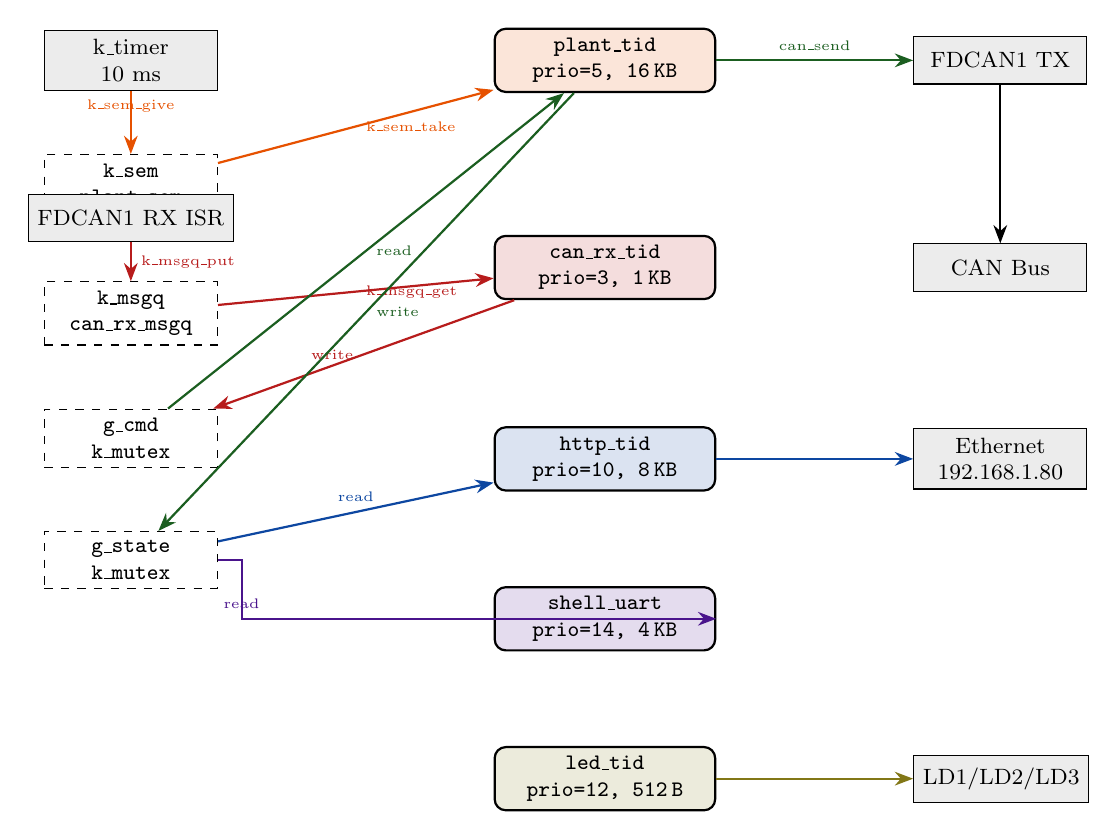
\begin{tikzpicture}[
  node distance=1.4cm and 2.2cm,
  thread/.style={rectangle, rounded corners=4pt, draw, thick, minimum width=2.8cm,
                 minimum height=0.75cm, font=\footnotesize\ttfamily, align=center},
  obj/.style={rectangle, draw, dashed, minimum width=2.2cm,
              minimum height=0.6cm, font=\footnotesize\ttfamily, align=center},
  hw/.style={rectangle, draw, fill=gray!15, minimum width=2.2cm,
             minimum height=0.6cm, font=\footnotesize, align=center},
  arr/.style={-Stealth, thick},
]

% Hardware / shared objects (left column)
\node[hw] (timer) {k\_timer\\\footnotesize 10 ms};
\node[obj, below=0.8cm of timer] (sem) {k\_sem\\plant\_sem};
\node[obj, below=0.8cm of sem] (msgq) {k\_msgq\\can\_rx\_msgq};
\node[obj, below=0.8cm of msgq] (gcmd) {g\_cmd\\k\_mutex};
\node[obj, below=0.8cm of gcmd] (gstate) {g\_state\\k\_mutex};

% Threads (right column)
\node[thread, fill=colTimer!15, right=3.5cm of timer] (plant)
  {plant\_tid\\\footnotesize prio=5, 16\,KB};
\node[thread, fill=colCAN!15, below=1.8cm of plant] (canrx)
  {can\_rx\_tid\\\footnotesize prio=3, 1\,KB};
\node[thread, fill=colHTTP!15, below=1.6cm of canrx] (http)
  {http\_tid\\\footnotesize prio=10, 8\,KB};
\node[thread, fill=colShell!15, below=1.2cm of http] (shell)
  {shell\_uart\\\footnotesize prio=14, 4\,KB};
\node[thread, fill=colLED!15, below=1.2cm of shell] (led)
  {led\_tid\\\footnotesize prio=12, 512\,B};

% ISR
\node[hw, above=0.5cm of msgq] (isr) {FDCAN1 RX ISR};

% External
\node[hw, right=2.5cm of plant] (fdtx) {FDCAN1 TX};
\node[hw, right=2.5cm of http] (eth) {Ethernet\\\footnotesize 192.168.1.80};
\node[hw, right=2.5cm of canrx] (bus) {CAN Bus};
\node[hw, right=2.5cm of led] (leds) {LD1/LD2/LD3};

% Arrows: timer chain
\draw[arr, colTimer] (timer) -- node[above, font=\tiny]{k\_sem\_give} (sem);
\draw[arr, colTimer] (sem) -- node[right, font=\tiny]{k\_sem\_take} (plant);

% Arrows: CAN RX chain
\draw[arr, colCAN] (isr) -- node[right, font=\tiny]{k\_msgq\_put} (msgq);
\draw[arr, colCAN] (msgq) -- node[right, font=\tiny]{k\_msgq\_get} (canrx);
\draw[arr, colCAN] (canrx) -- node[left, font=\tiny]{write} (gcmd);

% Arrows: plant reads/writes
\draw[arr, colPlant] (gcmd) -- node[right, font=\tiny]{read} (plant);
\draw[arr, colPlant] (plant) -- node[right, font=\tiny]{write} (gstate);

% Arrows: consumers
\draw[arr, colHTTP] (gstate) -- node[above, font=\tiny]{read} (http);
\draw[arr, colShell] (gstate.east) -- ++(0.3,0) |- node[above, font=\tiny]{read} (shell.east);

% Arrows: output
\draw[arr, colPlant] (plant) -- node[above, font=\tiny]{can\_send} (fdtx);
\draw[arr] (fdtx) -- (bus);
\draw[arr, colHTTP] (http) -- (eth);
\draw[arr, colLED] (led) -- (leds);

\end{tikzpicture}
\caption{Inter-thread communication in the Zephyr port. The plant thread sits
at the centre, consuming commands from the CAN~RX thread and publishing state
to the HTTP and shell threads.}
\label{fig:thread_arch}
\end{figure}

% =============================================================================
\section{Plant Loop Timing}
% =============================================================================

\subsection{Timer-Semaphore Pattern}

The plant loop does \emph{not} use \texttt{k\_msleep}. Instead it uses a
\textbf{hardware timer} (\texttt{k\_timer}) that fires every \SI{10}{ms} and
gives a binary semaphore. The plant thread blocks on \texttt{k\_sem\_take}
until the next tick arrives. This pattern ensures that the computation
\emph{budget} for one step is the full \SI{10}{ms} interval and that any
overrun is detected via a cycle counter.

\begin{lstlisting}[language=C++, caption={Timer-semaphore plant loop skeleton}]
K_SEM_DEFINE(plant_sem, 0, 1);
static void plant_timer_expiry(struct k_timer*) { k_sem_give(&plant_sem); }
K_TIMER_DEFINE(plant_timer, plant_timer_expiry, NULL);

static void plant_thread(void*, void*, void*)
{
    k_timer_start(&plant_timer, K_MSEC(10), K_MSEC(10));
    while (true) {
        k_sem_take(&plant_sem, K_FOREVER);          // blocks until next tick
        const uint32_t t0 = k_cycle_get_32();       // start of budget
        const double   t_s = k_uptime_get_32() / 1000.0;

        // --- physics step (see Section 5) ---
        s_plant.step(local_state, cmd, DT_S);

        // --- CAN TX ---
        can_tx_send_all(local_state, t_s, loop_us);

        const uint32_t dt = k_cycle_get_32() - t0;
        const uint32_t loop_us = k_cyc_to_us_ceil32(dt); // budget check
    }
}
K_THREAD_DEFINE(plant_tid, 16384, plant_thread, NULL, NULL, NULL, 5, 0, 0);
\end{lstlisting}

\subsection{Timing Budget}

\begin{center}
\begin{tabular}{lrl}
\toprule
Activity & Typical cost & Notes \\
\midrule
Mutex lock/unlock (×4) & \SI{<1}{\micro s} & \texttt{g\_cmd}, \texttt{g\_state} \\
Physics step (\texttt{s\_plant.step}) & 200--\SI{400}{\micro s} & Dugoff + 3-DOF + battery \\
CAN TX (15 frames) & 150--\SI{250}{\micro s} & \texttt{can\_send} non-blocking \\
Brake diagnostics log & \SI{<10}{\micro s} & Only when \texttt{brake\_cmd\_pct > 1} \\
\textbf{Total} & \textbf{\SI{<700}{\micro s}} & Budget: \SI{10000}{\micro s} \\
\bottomrule
\end{tabular}
\end{center}

The \SI{10}{ms} budget is comfortably satisfied. The remaining \SI{9.3}{ms}
is spent in \texttt{k\_sem\_take} waiting for the next tick, during which
the Cortex-M7 is idle and lower-priority threads (HTTP, LED, shell) run.

\subsection{Timing Flow}

\begin{figure}[H]
\centering
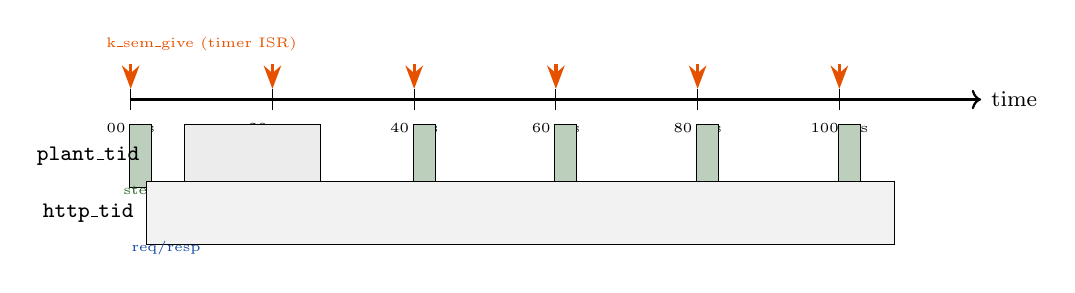
\begin{tikzpicture}[
  scale=0.9,
  arr/.style={-Stealth, thick},
  tick/.style={draw, fill=colTimer!30, minimum height=0.8cm, minimum width=1.6cm,
               font=\footnotesize, align=center},
  work/.style={draw, fill=colPlant!30, minimum height=0.8cm, font=\footnotesize, align=center},
  idle/.style={draw, fill=gray!15, minimum height=0.8cm, font=\footnotesize, align=center},
]
% Timeline
\draw[thick, ->] (0,0) -- (12,0) node[right]{\footnotesize time};

% Tick marks at 0, 2, 4 (scaled: 10ms = 2cm)
\foreach \x in {0, 2, 4, 6, 8, 10} {
  \draw (\x, -0.15) -- (\x, 0.15);
  \node[below, font=\tiny] at (\x, -0.2) {\x0 ms};
}

% k_timer gives sem (vertical arrows)
\foreach \x in {0, 2, 4, 6, 8, 10} {
  \draw[arr, colTimer, very thick] (\x, 0.5) -- (\x, 0.15);
}
\node[above, font=\tiny, colTimer] at (1, 0.55) {k\_sem\_give (timer ISR)};

% plant_tid: work block then idle
\foreach \x in {0, 2, 4, 6, 8, 10} {
  \node[work, minimum width=0.28cm] at (\x+0.14, -0.8) {};
}
\node[idle, minimum width=1.72cm] at (0.14+0.86+0.72, -0.8) {};
% Labels
\node[font=\tiny, colPlant] at (0.14, -1.3) {step};
\node[font=\tiny, gray] at (1, -1.3) {idle};
\node[font=\tiny] at (-0.6, -0.8) {\footnotesize\ttfamily plant\_tid};

% HTTP thread: periodic accept/send
\node[work, fill=colHTTP!30, minimum width=0.5cm] at (0.5, -1.6) {};
\node[idle, fill=gray!10, minimum width=9.5cm] at (5.5, -1.6) {};
\node[font=\tiny] at (-0.6, -1.6) {\footnotesize\ttfamily http\_tid};
\node[font=\tiny, colHTTP] at (0.5, -2.1) {req/resp};

\end{tikzpicture}
\caption{Simplified timing diagram showing the \SI{10}{ms} plant step and the
longer HTTP request/response event. The Cortex-M7 is idle between steps.}
\label{fig:timing}
\end{figure}

% =============================================================================
\section{CAN Architecture}
% =============================================================================

\subsection{CAN RX Path}

\begin{figure}[H]
\centering
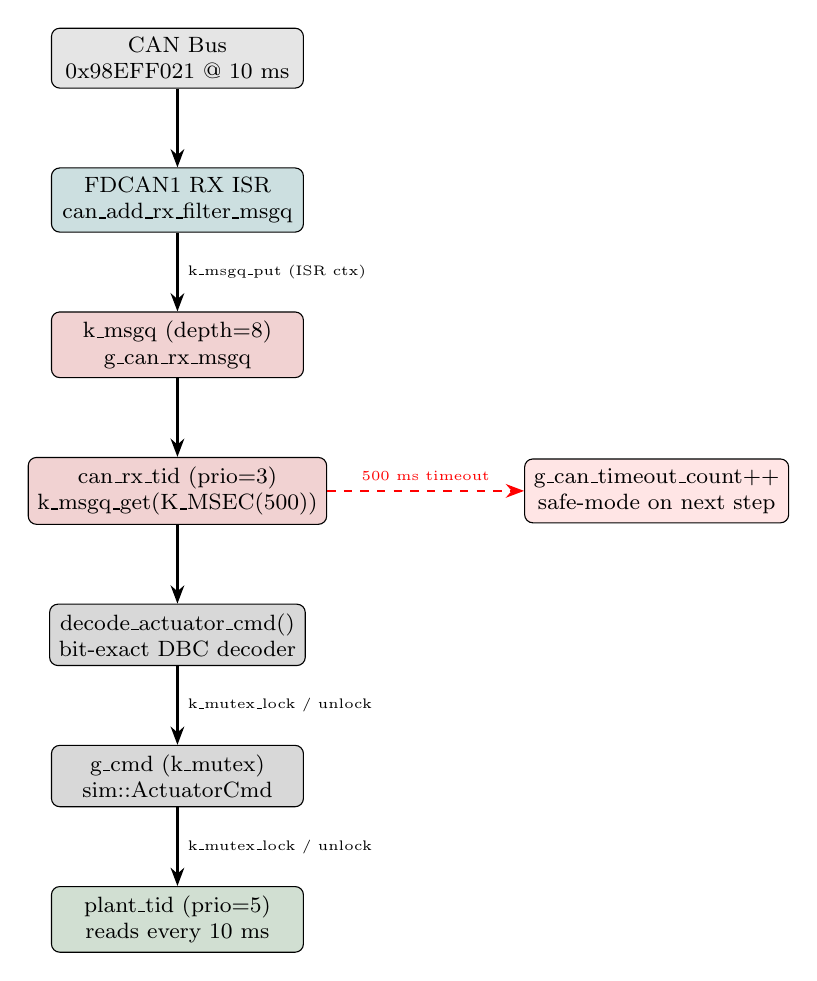
\begin{tikzpicture}[
  node distance=1.0cm and 2.5cm,
  box/.style={rectangle, draw, rounded corners=3pt, minimum width=3.2cm,
              minimum height=0.7cm, font=\footnotesize, align=center},
  arr/.style={-Stealth, thick},
]

\node[box, fill=gray!20] (bus) {CAN Bus\\\footnotesize 0x98EFF021 @ 10 ms};
\node[box, fill=colISR!20, below=of bus] (isr) {FDCAN1 RX ISR\\\footnotesize can\_add\_rx\_filter\_msgq};
\node[box, fill=colCAN!20, below=of isr] (msgq) {k\_msgq (depth=8)\\\footnotesize g\_can\_rx\_msgq};
\node[box, fill=colCAN!20, below=of msgq] (rx) {can\_rx\_tid (prio=3)\\\footnotesize k\_msgq\_get(K\_MSEC(500))};
\node[box, fill=colMutex!20, below=of rx] (decode) {decode\_actuator\_cmd()\\\footnotesize bit-exact DBC decoder};
\node[box, fill=colMutex!20, below=of decode] (gcmd) {g\_cmd (k\_mutex)\\\footnotesize sim::ActuatorCmd};
\node[box, fill=colPlant!20, below=of gcmd] (plant) {plant\_tid (prio=5)\\\footnotesize reads every 10 ms};

\draw[arr] (bus) -- (isr);
\draw[arr] (isr) -- node[right, font=\tiny]{k\_msgq\_put (ISR ctx)} (msgq);
\draw[arr] (msgq) -- (rx);
\draw[arr] (rx) -- (decode);
\draw[arr] (decode) -- node[right, font=\tiny]{k\_mutex\_lock / unlock} (gcmd);
\draw[arr] (gcmd) -- node[right, font=\tiny]{k\_mutex\_lock / unlock} (plant);

% Timeout branch
\node[box, fill=red!10, right=2.5cm of rx] (timeout) {g\_can\_timeout\_count++\\\footnotesize safe-mode on next step};
\draw[arr, dashed, red] (rx) -- node[above, font=\tiny]{500 ms timeout} (timeout);

\end{tikzpicture}
\caption{CAN RX data path from bus to plant thread. The ISR deposits frames
into a message queue; \texttt{can\_rx\_tid} decodes them. A 500\,ms timeout
triggers safe-mode in the plant thread.}
\label{fig:can_rx}
\end{figure}

The inline decoder reads directly from the 8-byte \texttt{zf.data[]} array,
using the bit positions from the DBC:

\begin{lstlisting}[language=C++, caption={ACTUATOR\_CMD\_1 inline decoder}]
// Intel byte order (LSB-first), positions from can_map.dbc:
c.system_enable       = (d[0] >> 0) & 0x01;
c.gear_position       = static_cast<GearPosition>((d[0] >> 1) & 0x03);
c.steer_cmd_deg       = (int16_t)(d[1] | (d[2] << 8)) * 0.1;
c.drive_torque_cmd_nm = (int16_t)(d[3] | (d[4] << 8)) * 10.0;
c.brake_cmd_pct       = d[5] * 1.0;
\end{lstlisting}

\subsection{CAN TX Path}

\texttt{can\_tx.cpp} is called once per \SI{10}{ms} plant step. It packs all
15 TX frames from the \texttt{PlantState} fields and calls \texttt{can\_send()}
for each frame that is due (modulo the frame's \texttt{cycle\_ms} period):

\begin{lstlisting}[language=C++, caption={CAN TX dispatch loop (simplified)}]
void can_tx_send_all(const plant::PlantState& s, double t_s, uint32_t loop_us)
{
    for (uint8_t i = 0; i < can_static::k_tx_frame_count; ++i) {
        const auto& fd = can_static::k_frames[i];
        if (!fd.is_rx && should_send(i, t_s)) {
            can_pack_and_send(fd, s, t_s, loop_us);
        }
    }
}
\end{lstlisting}

\begin{center}
\begin{tabular}{llrr}
\toprule
Frame & 29-bit ID & Signals & Rate \\
\midrule
\texttt{ACTUATOR\_CMD\_1} & \texttt{0x98EFF021} & 6 & RX 10 ms \\
\texttt{IMU\_ACC} & \texttt{0x8CFF0028} & 4 & TX 5 ms \\
\texttt{VEHICLE\_STATE\_1} & \texttt{0x98FF50F0} & 4 & TX 10 ms \\
\texttt{WHEEL\_SPEED} & \texttt{0x98FF3040} & 4 & TX 10 ms \\
\texttt{GNSS\_LL} & \texttt{0x98FF1029} & 2 & TX 100 ms \\
\ldots & \ldots & \ldots & \ldots \\
\bottomrule
\end{tabular}
\end{center}

\subsection{CAN Watchdog / Safe-Mode}

The plant thread compares the current uptime against \texttt{g\_last\_rx\_t}
(updated by \texttt{can\_rx\_tid} on every decoded frame). If the gap exceeds
\SI{500}{ms}, the command is replaced by a zeroed \texttt{ActuatorCmd}:

\begin{lstlisting}[language=C++, caption={Watchdog in plant thread}]
if ((t_s - g_last_rx_t) > 0.5) {
    cmd = sim::ActuatorCmd{};  // zero torque, zero brake, neutral gear
}
\end{lstlisting}

This prevents the vehicle from running away when the CAN controller disconnects.
\texttt{g\_can\_timeout\_count} is displayed on the web dashboard under
\emph{CAN Stats} and accessible via the \texttt{can stats} shell command.

% =============================================================================
\section{Physics on the MCU}
% =============================================================================

\subsection{Subsystem Execution Order}

The \texttt{PlantModel::step()} call invokes five subsystems via the
\texttt{SubsystemManager} visitor in fixed priority order:

\begin{figure}[H]
\centering
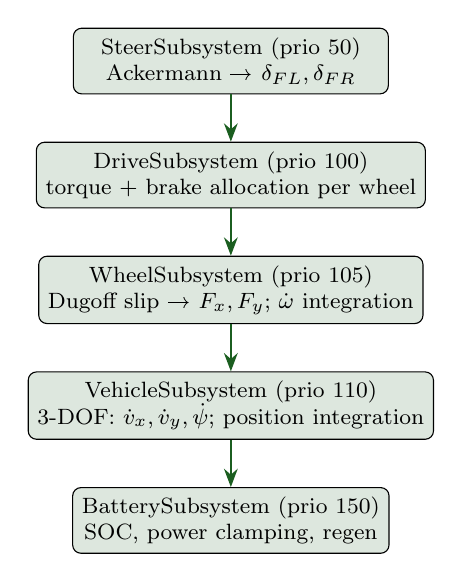
\begin{tikzpicture}[
  node distance=0.6cm,
  sub/.style={rectangle, draw, rounded corners=3pt, fill=colPlant!15,
              minimum width=4cm, minimum height=0.65cm, font=\footnotesize, align=center},
  arr/.style={-Stealth, thick, colPlant},
]
\node[sub] (steer) {SteerSubsystem (prio 50)\\\footnotesize Ackermann → $\delta_{FL},\delta_{FR}$};
\node[sub, below=of steer] (drive) {DriveSubsystem (prio 100)\\\footnotesize torque + brake allocation per wheel};
\node[sub, below=of drive] (wheel) {WheelSubsystem (prio 105)\\\footnotesize Dugoff slip → $F_x,F_y$; $\dot{\omega}$ integration};
\node[sub, below=of wheel] (vehicle) {VehicleSubsystem (prio 110)\\\footnotesize 3-DOF: $\dot{v}_x,\dot{v}_y,\dot{\psi}$; position integration};
\node[sub, below=of vehicle] (batt) {BatterySubsystem (prio 150)\\\footnotesize SOC, power clamping, regen};

\draw[arr] (steer) -- (drive);
\draw[arr] (drive) -- (wheel);
\draw[arr] (wheel) -- (vehicle);
\draw[arr] (vehicle) -- (batt);
\end{tikzpicture}
\caption{Subsystem execution order within one \SI{10}{ms} step. Each subsystem
reads from and writes to the shared \texttt{PlantState} struct.}
\label{fig:subsystems}
\end{figure}

\subsection{Heavy-Duty Electric Vehicle Parameters}

\begin{center}
\begin{tabular}{lrl}
\toprule
Parameter & Value & Notes \\
\midrule
Mass & \SI{218000}{kg} & 218~t (payload loaded) \\
Wheel radius & \SI{1.93}{m} & \\
Motor torque max & \SI{145000}{N.m} & \\
Motor power max & \SI{2013}{kW} & \\
Gear ratio & 28.0 & motor to wheel \\
Drivetrain efficiency & 0.92 & \\
Brake torque max & \SI{2.5e6}{N.m} & 2.5~MNm $\to$ $\approx 0.6\,g$ \\
Aerodynamic drag $c_d$ & 1.85 & \\
Rolling resistance $F_\text{roll}$ & \SI{9500}{N} & \\
Max speed & \SI{17.78}{m.s^{-1}} & 64~km/h \\
Dugoff $C_x$ base & \SI{280000}{N} & load-scaled: $(F_z/F_{z,\text{ref}})^{0.5}$ \\
Dugoff $C_y$ base & \SI{220000}{N} & \\
Reference normal load $F_{z,\text{ref}}$ & \SI{800000}{N} & \\
Peak friction $\mu$ (default) & 0.72 & compact gravel \\
\bottomrule
\end{tabular}
\end{center}

\subsection{Braking Performance}

At full brake (\texttt{brake\_cmd\_pct = 100}), the torque budget per wheel is:

\begin{equation}
  \tau_{\text{brake,wheel}} = \frac{\tau_{\text{max}}}{4} = \frac{2.5 \times 10^6}{4} = \SI{625000}{N.m}
\end{equation}

The equilibrium wheel-level braking force (Dugoff slip-limited) is:

\begin{equation}
  F_{x,\text{brk}} = \frac{\tau_{\text{brake,wheel}}}{R} = \frac{625000}{1.93} \approx \SI{323800}{N} \text{ per wheel}
\end{equation}

Total deceleration:

\begin{equation}
  a_{\text{brk}} = \frac{4 \times F_{x,\text{brk}}}{m} = \frac{4 \times 323800}{218000} \approx \SI{5.94}{m.s^{-2}} \approx 0.61\,g
\end{equation}

This is below the tyre friction ceiling
($\mu F_z = 0.72 \times \SI{535000}{N} \approx \SI{385000}{N}$ per wheel),
so the wheels do not lock. The brake diagnostics log confirms
$a \approx -5.9\,\text{m/s}^2$ during full braking.

% =============================================================================
\section{Shared State and Concurrency}
% =============================================================================

\subsection{Global State}

All inter-thread data lives in a small set of globals defined in
\texttt{main.cpp}:

\begin{lstlisting}[language=C++, caption={Shared globals in main.cpp}]
plant::PlantState  g_state{};    // guarded by g_state_mutex
sim::ActuatorCmd   g_cmd{};      // guarded by g_cmd_mutex
K_MUTEX_DEFINE(g_state_mutex);
K_MUTEX_DEFINE(g_cmd_mutex);

volatile uint32_t  g_can_tx_count   = 0;
volatile uint32_t  g_can_rx_count   = 0;
volatile uint32_t  g_can_timeout_count = 0;
volatile double    g_last_rx_t      = 0.0;
double             g_surface_mu     = 0.72;
\end{lstlisting}

\subsection{Access Pattern}

\begin{center}
\begin{tabular}{lll}
\toprule
Global & Writers & Readers \\
\midrule
\texttt{g\_state} & \texttt{plant\_tid} & \texttt{http\_tid}, \texttt{shell\_uart} \\
\texttt{g\_cmd} & \texttt{can\_rx\_tid} & \texttt{plant\_tid} \\
\texttt{g\_last\_rx\_t} & \texttt{can\_rx\_tid}, \texttt{http\_tid} & \texttt{plant\_tid} \\
\texttt{g\_surface\_mu} & \texttt{shell\_uart} & \texttt{plant\_tid} \\
\texttt{g\_can\_tx\_count} & \texttt{plant\_tid} & \texttt{http\_tid}, \texttt{shell\_uart} \\
\texttt{g\_can\_rx\_count} & \texttt{can\_rx\_tid} & \texttt{http\_tid}, \texttt{shell\_uart} \\
\bottomrule
\end{tabular}
\end{center}

Critical sections are kept short: the mutex is locked only for the duration of
a struct copy (\texttt{g\_state = local\_state}), never during the physics
computation itself.

% =============================================================================
\section{HTTP Dashboard}
% =============================================================================

\subsection{Module Structure}

The HTTP module is split across six files for maintainability:

\begin{center}
\begin{tabular}{ll}
\toprule
File & Responsibility \\
\midrule
\texttt{http\_server.cpp} & Socket lifecycle: \texttt{socket→bind→listen→accept→close} \\
\texttt{http\_cmd.cpp} & Request-line parse, query-string decode, \texttt{apply\_web\_cmd()} \\
\texttt{http\_page.cpp} & HTML page builder — all \texttt{snprintf} / \texttt{send\_str} calls \\
\texttt{http\_html.hpp} & Static HTML fragments as \texttt{const char[]} constants \\
\texttt{dashboard.css} & All CSS rules as a real \texttt{.css} file (no C escaping) \\
\texttt{http\_internal.hpp} & Shared internal declarations across the three \texttt{.cpp} files \\
\bottomrule
\end{tabular}
\end{center}

\subsection{CSS Embedding}

\texttt{dashboard.css} is a plain CSS file editable with any editor or IDE with
CSS support. It is converted to a C byte array at build time by Zephyr's
\texttt{generate\_inc\_file\_for\_target()} CMake function:

\begin{lstlisting}[language={[LaTeX]TeX}, caption={CMakeLists.txt — CSS embedding}]
generate_inc_file_for_target(app
    ${CMAKE_CURRENT_SOURCE_DIR}/src/http/dashboard.css
    ${CMAKE_CURRENT_BINARY_DIR}/dashboard.css.inc
)
\end{lstlisting}

\begin{lstlisting}[language=C++, caption={http\_page.cpp — including the generated array}]
static const char kDashboardCss[] = {
#include "dashboard.css.inc"   // comma-separated hex bytes from file2hex.py
    '\0'
};
\end{lstlisting}

Incremental builds detect changes to \texttt{dashboard.css} and regenerate the
\texttt{.inc} file automatically; only \texttt{http\_page.cpp} needs
recompilation.

\subsection{Request Flow}

\begin{figure}[H]
\centering
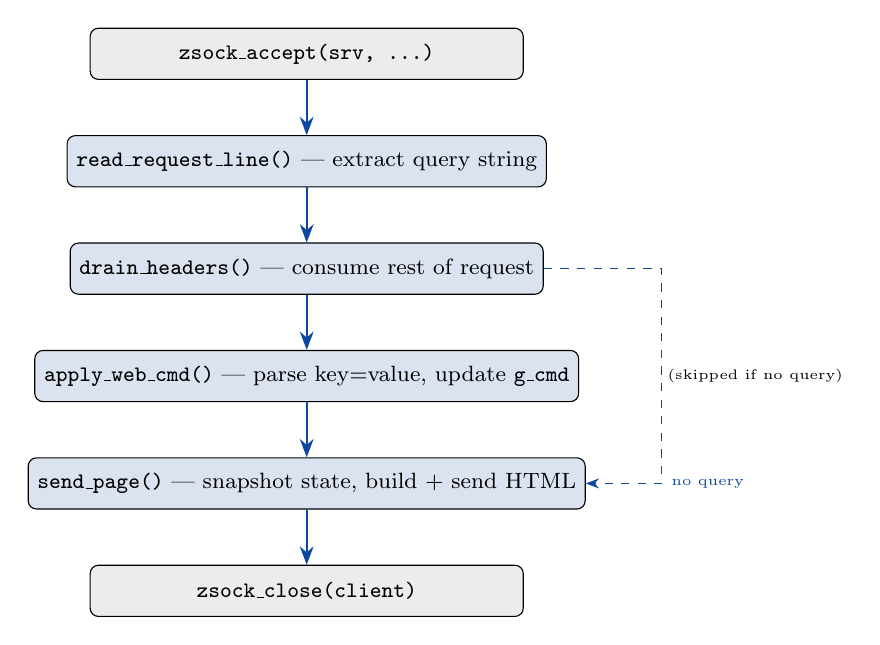
\begin{tikzpicture}[
  node distance=0.7cm and 0,
  box/.style={rectangle, draw, rounded corners=3pt, minimum width=5.5cm,
              minimum height=0.65cm, font=\footnotesize, align=center},
  arr/.style={-Stealth, thick, colHTTP},
]
\node[box, fill=gray!15] (accept) {\texttt{zsock\_accept(srv, \ldots)}};
\node[box, fill=colHTTP!15, below=of accept] (req) {\texttt{read\_request\_line()} — extract query string};
\node[box, fill=colHTTP!15, below=of req] (drain) {\texttt{drain\_headers()} — consume rest of request};
\node[box, fill=colHTTP!15, below=of drain] (cmd) {\texttt{apply\_web\_cmd()} — parse key=value, update \texttt{g\_cmd}};
\node[box, fill=colHTTP!15, below=of cmd] (page) {\texttt{send\_page()} — snapshot state, build + send HTML};
\node[box, fill=gray!15, below=of page] (close) {\texttt{zsock\_close(client)}};

\draw[arr] (accept) -- (req);
\draw[arr] (req) -- (drain);
\draw[arr] (drain) -- (cmd);
\draw[arr] (cmd) -- (page);
\draw[arr] (page) -- (close);

% Optional branch: no query string
\node[font=\tiny, right=1cm of cmd] (skip) {(skipped if no query)};
\draw[-Stealth, dashed, colHTTP] (drain.east) -| ++(1.5,0) |- node[right, font=\tiny]{no query} (page.east);

\end{tikzpicture}
\caption{HTTP server request lifecycle for one browser connection.}
\label{fig:http_flow}
\end{figure}

\subsection{Dashboard Cards}

\begin{enumerate}[leftmargin=*]
  \item \textbf{Plant State} — $v_x$, $v_y$, yaw, yaw rate, position, steer
        angle, SOC, per-wheel $\omega$, surface~$\mu$
  \item \textbf{Actuator Command} — enable, gear, torque, brake, steer (current
        command sent to plant)
  \item \textbf{CAN Stats} — TX frames, RX frames, timeout count, last RX
        timestamp
  \item \textbf{Controls} — quick-action buttons (STOP, Drive FWD, Drive REV,
        steer $\pm 5^\circ$) and a manual-inject form; all via HTTP GET
  \item \textbf{Kernel Threads} — per-thread name, priority, stack used/total
        (via \texttt{k\_thread\_foreach})
  \item \textbf{Vehicle Info} — hardcoded Heavy-Duty Electric Vehicle specification table
\end{enumerate}

% =============================================================================
\section{Shell Commands}
% =============================================================================

All commands are implemented in \texttt{shell/debug\_cmds.cpp} using Zephyr's
\texttt{SHELL\_CMD\_REGISTER} macro.

\begin{center}
\begin{tabular}{ll}
\toprule
Command & Action \\
\midrule
\texttt{plant state} & Dump all \texttt{PlantState} fields \\
\texttt{plant inject <steer> <torque> <brake>} & Inject actuator command directly \\
\texttt{plant mu <val>} & Set surface friction coefficient (0.1–1.0) \\
\texttt{plant reset} & Zero all plant state \\
\texttt{can stats} & TX/RX frame counts, timeouts, last RX timestamp \\
\texttt{can rx\_frame} & Last decoded \texttt{ACTUATOR\_CMD\_1} fields \\
\texttt{can tx\_test <steer> <torque> <brake>} & Encode + transmit test frame (loopback) \\
\texttt{can map} & Print static CAN frame table (16 entries) \\
\texttt{vehicle info} & Heavy-Duty Electric Vehicle parameters + live surface~$\mu$ \\
\texttt{network mac} & MAC and IP from \texttt{net\_if\_get\_default()} \\
\texttt{system uptime} & HH:MM:SS and ms \\
\bottomrule
\end{tabular}
\end{center}

% =============================================================================
\section{Memory Layout}
% =============================================================================

\subsection{Measured Flash Footprint}

Measured with \texttt{west build -t rom\_report} on a full Phase~4 build.
Total Flash: \textbf{\SI{236957}{B} $\approx$ \SI{231.4}{KB}}
--- \textbf{11.3\,\%} of the \SI{2}{MB} Flash budget; \SI{1.77}{MB} free.

\begin{center}
\begin{tabular}{lrrl}
\toprule
Region & Budget & Measured & Notes \\
\midrule
Total Flash & \SI{2}{MB} & \SI{231.4}{KB} & 11.3\,\% utilised \\
\addlinespace
App (\texttt{zephyr/src/}) & --- & \SI{12.7}{KB} & threads, HTTP, CAN, shell \\
\quad \texttt{can/can\_tx.cpp} & --- & \SI{3416}{B} & \texttt{can\_tx\_send\_all()} \\
\quad \texttt{shell/debug\_cmds.cpp} & --- & \SI{2372}{B} & 11 command handlers \\
\quad \texttt{plant/plant\_thread.cpp} & --- & \SI{1488}{B} & \texttt{plant\_thread()} \\
\quad \texttt{http/http\_page.cpp} & --- & \SI{1642}{B} & \texttt{send\_page()} \\
\quad \texttt{kDashboardCss} (rodata) & --- & \SI{1758}{B} & embedded CSS \\
Shared plant physics & --- & \SI{12.8}{KB} & subsystems from \texttt{src/plant/} \\
Zephyr RTOS & --- & \SI{121.1}{KB} & kernel + subsys + drivers \\
Newlib / unresolved & --- & \SI{61.5}{KB} & math, C stdlib \\
\bottomrule
\end{tabular}
\end{center}

\subsection{Measured RAM Footprint}

Measured with \texttt{west build -t ram\_report} on a full Phase~4 build
targeting \texttt{nucleo\_h753zi}.
Total static RAM: \textbf{\SI{241075}{B} $\approx$ \SI{235}{KB}}
--- \textbf{22.9\,\%} of the \SI{1}{MB} SRAM budget; \SI{765}{KB} free.

\begin{center}
\begin{tabular}{lrrl}
\toprule
Region & Budget & Measured & Dominant item \\
\midrule
Total SRAM & \SI{1}{MB} & \SI{235}{KB} (241\,075\,B) & 22.9\,\% utilised \\
\addlinespace
App code & --- & \SI{27.4}{KB} (28\,100\,B) & stacks + shared state \\
\quad \texttt{plant\_thread.cpp} & --- & \SI{16760}{B} & stack 16\,448\,B \\
\quad \texttt{http\_server.cpp} & --- & \SI{8488}{B} & stack 8\,256\,B \\
\quad \texttt{can\_rx.cpp} & --- & \SI{1372}{B} & stack 1\,088\,B + msgq \\
\quad \texttt{led\_task.cpp} & --- & \SI{808}{B} & stack 576\,B \\
\quad \texttt{main.cpp} & --- & \SI{672}{B} & \texttt{g\_state} 560\,B \\
\addlinespace
Zephyr kernel & --- & \SI{133.6}{KB} & \texttt{kheap} 128\,KB \\
Networking subsystem & --- & \SI{34.0}{KB} & TCP slab, pkt/buf pools \\
ETH driver & --- & \SI{14.5}{KB} & DMA RX+TX buffers$^*$ \\
Logging subsystem & --- & \SI{5.5}{KB} & ring buffer + thread \\
\bottomrule
\end{tabular}
\end{center}

\noindent $^*$ ETH DMA buffers reside in a dedicated \texttt{eth\_stm32} SRAM
region at \texttt{0x30040000}, separate from the main AXI SRAM.

\medskip
\noindent\textbf{Heap:} \texttt{kheap\_\_system\_heap} = \SI{128}{KB}
(configured pool). Runtime peak is inspectable via the Zephyr shell:

\begin{lstlisting}[language=bash]
uart:~$ kernel heap
\end{lstlisting}

\noindent If RAM becomes constrained, reduce \texttt{CONFIG\_HEAP\_MEM\_POOL\_SIZE}
in \texttt{prj.conf}; \SI{64}{KB} is sufficient for current allocations.

\subsection{Thread Stack Allocation (Actual)}

Zephyr adds alignment padding to each \texttt{K\_THREAD\_DEFINE} stack;
the table below shows the aligned sizes from \texttt{ram\_report}.

\begin{center}
\begin{tabular}{lrrl}
\toprule
Thread & Configured & Actual & Base address \\
\midrule
\texttt{plant\_tid} & \SI{16384}{B} & \SI{16448}{B} & \texttt{0x24008080} \\
\texttt{http\_tid}  & \SI{8192}{B}  & \SI{8256}{B}  & \texttt{0x24005c00} \\
\texttt{z\_main\_stack} & \SI{4096}{B} & \SI{4160}{B} & \texttt{0x2400ecc0} \\
\texttt{z\_interrupt\_stacks} & \SI{2048}{B} & \SI{2112}{B} & \texttt{0x2400e300} \\
\texttt{can\_rx\_tid} & \SI{1024}{B} & \SI{1088}{B} & \texttt{0x24007c40} \\
\texttt{sys\_work\_q} & \SI{1024}{B} & \SI{1088}{B} & \texttt{0x2400fd00} \\
\texttt{logging}     & \SI{1024}{B} & \SI{1088}{B} & \texttt{0x2400c0c0} \\
\texttt{led\_tid}    & \SI{512}{B}  & \SI{576}{B}  & \texttt{0x240059c0} \\
\texttt{z\_idle\_stacks} & \SI{320}{B} & \SI{384}{B} & \texttt{0x2400eb40} \\
\midrule
\textbf{Total} & --- & \textbf{\SI{35200}{B} ($\approx$\SI{34.4}{KB})} & \\
\bottomrule
\end{tabular}
\end{center}

\subsection{Audit Commands}

\begin{lstlisting}[language=bash, caption={RAM and Flash audit}]
west build -t ram_report   # per-object static RAM
west build -t rom_report   # per-object Flash (.text + .rodata)
uart:~$ kernel heap        # runtime heap peak (Zephyr shell)
\end{lstlisting}

% =============================================================================
\section{Build System}
% =============================================================================

\subsection{Dual Build Paths}

Both the host simulator and the embedded firmware compile from the same
\texttt{src/} and \texttt{utils/} source tree. Only \texttt{CMakeLists.txt}
and the platform source files differ.

\begin{figure}[H]
\centering
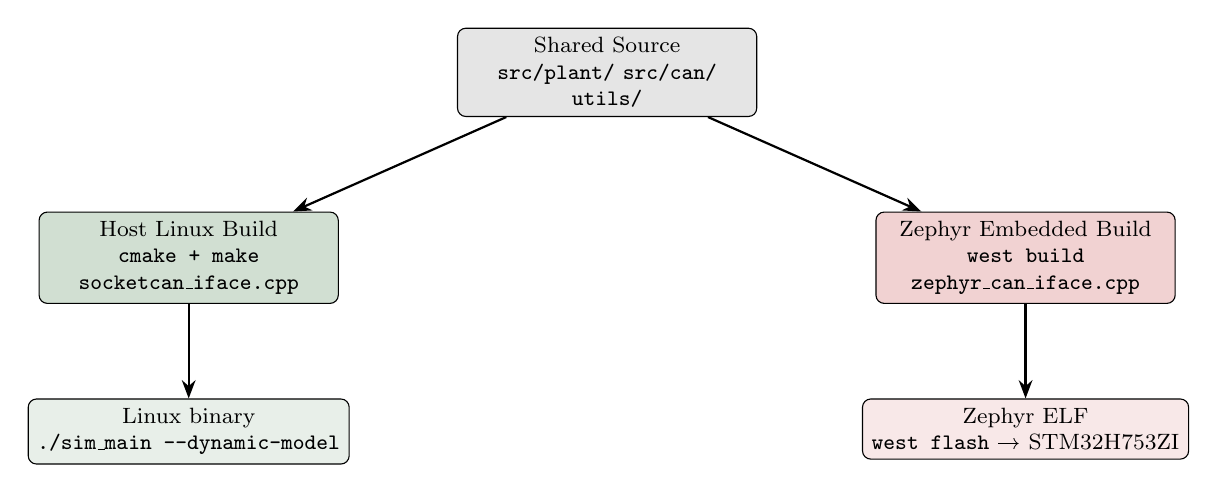
\begin{tikzpicture}[
  node distance=1.2cm and 3cm,
  box/.style={rectangle, draw, rounded corners=3pt, minimum width=3.8cm,
              minimum height=0.65cm, font=\footnotesize, align=center},
  arr/.style={-Stealth, thick},
]
\node[box, fill=gray!20] (shared) {Shared Source\\\texttt{src/plant/}  \texttt{src/can/}\\\texttt{utils/}};
\node[box, fill=colPlant!20, below left=1.2cm and 1.5cm of shared] (host)
  {Host Linux Build\\\texttt{cmake + make}\\\texttt{socketcan\_iface.cpp}};
\node[box, fill=colCAN!20, below right=1.2cm and 1.5cm of shared] (emb)
  {Zephyr Embedded Build\\\texttt{west build}\\\texttt{zephyr\_can\_iface.cpp}};

\draw[arr] (shared) -- (host);
\draw[arr] (shared) -- (emb);

\node[box, fill=colPlant!10, below=of host] (bin1) {Linux binary\\\texttt{./sim\_main --dynamic-model}};
\node[box, fill=colCAN!10, below=of emb] (bin2) {Zephyr ELF\\\texttt{west flash} → STM32H753ZI};

\draw[arr] (host) -- (bin1);
\draw[arr] (emb) -- (bin2);
\end{tikzpicture}
\caption{Dual build paths sharing the same plant and CAN source.}
\label{fig:build}
\end{figure}

\subsection{Build Commands}

\begin{lstlisting}[language=bash, caption={Complete clean build and flash sequence}]
cd ~/zephyrproject
rm -rf build                       # required when prj.conf or overlay changes
west build -b nucleo_h753zi \
    ~/repos/vehicle-Dynamics-Sim-Can/zephyr
west flash
picocom -b 115200 /dev/ttyACM0     # UART shell monitor
\end{lstlisting}

Dashboard is available at \texttt{http://192.168.1.80} once the Ethernet
link is up (typically within 2–3 s of boot).

% =============================================================================
\section{Verification}
% =============================================================================

\begin{enumerate}[leftmargin=*]
  \item \textbf{Boot banner} — UART shows:
    \begin{verbatim}
*** Booting Zephyr OS build v3.7.0 ***
[INF] hdv_sim: Heavy-Duty Electric Vehicle plant thread started (dt=10 ms, prio=5)
    \end{verbatim}

  \item \textbf{Plant state} — shell command \texttt{plant state} shows live
    $v_x$, yaw, SOC, wheel speeds; values change after \texttt{plant inject}.

  \item \textbf{CAN RX} — connect a CAN controller, send
    \texttt{ACTUATOR\_CMD\_1} at 10~ms; \texttt{can rx\_frame} shows decoded
    fields; \texttt{can stats} shows incrementing RX count.

  \item \textbf{CAN TX} — CAN analyzer on bus shows 15~TX frames at the
    rates in the DBC (5~ms IMU, 10~ms VEHICLE\_STATE, 100~ms GNSS, \ldots).

  \item \textbf{Web dashboard} — browser at \texttt{http://192.168.1.80}:
    \begin{itemize}[leftmargin=*]
      \item \emph{Drive FWD} button → $v_x$ rises toward \SI{17.78}{m.s^{-1}}
      \item \emph{STOP} button → $a_\text{long} \approx -5.9\,\text{m/s}^2$
            ($\approx 0.6\,g$)
      \item Kernel Threads card shows all thread names and stack usage
    \end{itemize}

  \item \textbf{Brake diagnostics} — UART log during hard braking:
    \begin{verbatim}
[brk] t=12.34 vx=8.320 a=-5.91 Fx=-1291kN tau=-2500kNm mode=dyn
[brk] omega FL=4.31 FR=4.31 RL=4.31 RR=4.31 ref=4.31 rad/s
    \end{verbatim}

  \item \textbf{Safe-mode} — disconnect the CAN controller; within 500~ms
    the \emph{CAN Stats} timeout counter increments and torque drops to zero.
\end{enumerate}

% =============================================================================
\section{Conclusion}
% =============================================================================

The Zephyr port demonstrates that a high-fidelity vehicle dynamics model
(3-DOF rigid body, Dugoff tyre, per-wheel rotational dynamics, Ackermann
steering, battery model) can execute deterministically on a mid-range
Cortex-M7 microcontroller with a \SI{10}{ms} timestep, leaving over 93\% of
the \SI{10}{ms} budget unused.

The dual build architecture — shared \texttt{src/plant/} compiled for both
Linux and Zephyr — minimises code divergence and allows the same test vectors
to be applied to both the host simulation and the embedded target. The web
dashboard, UART shell, and brake diagnostics provide sufficient observability
for iterative tuning without a full CAN analysis setup.

\end{document}
